\chapter{bullet}
\label{sec:bullet}
\lstset{style=68KStyle}

The player's bullet in Tempest 2000 is something of an outlier compared to all the other graphics in the game.
For some reason, it is not a polygon constructed from a data structure like the flipper or the player's claw.
Instead it is pinched directly from a spritesheet, 'beasty3.cry'. Take a look at the sheet and see if you can
spot the bullet:
\begin{figure}[H]
    \centering
    \begin{adjustbox}{width=12cm,center}
      \frame{
\includegraphics[width=12cm]{src/cry/beasty3.png}}%
    \end{adjustbox}
\caption{\icode{beasty3.cry}, with a bullet in there somewhere - can you find it?}
\end{figure}

\begin{lstlisting}
; *******************************************************************
; draw_pixex
; Draws a pixel based explosion.
; A member of the draw_vex and solids list.
; Called during the draw_objects sequence as a member of the draw_vex list.
; Called during the draw_objects sequence as a member of the solids list.
; *******************************************************************
draw_pixex:
    move.l #4,gpu_mode    ; Use the 'rex' routine in camel.gas.
    lea in_buf,a0         ; Point our GPU RAM input buffer at a0.
    move.l #pic,(a0)+     ; Use 'pic' (beasty3.cry) as our sprite sheet.
    move.l 36(a6),(a0)+   ; Y/X position within the 'pic' sprite sheet.
    move.l 46(a6),(a0)+   ; Width and height to pluck from the sheet.
    move.l 42(a6),d0      ; Put the scale in d0.
    asr.l #2,d0           ; Divide by 4.
    move.l d0,(a0)+       ; Add the x-scale to our GPU RAM input buffer.
    move.l d0,(a0)+       ; Add the y-scale to our GPU RAM input buffer.
    move.l #0,(a0)+       ; Add no shear to the input buffer.
    move.l #0,(a0)+
    move.l #1,(a0)+       ; Add Mode 1 = Centered to input buffer.
    move.l 4(a6),d0       ; Get the source X position.
    sub.l vp_x,d0         ; Subtract the player/camera viewpoint X position.
    move.l d0,(a0)+       ; Add it to our GPU RAM input buffer.
    move.l 8(a6),d0       ; Get the object's Y position.
    sub.l vp_y,d0         ; Subtract the player/camera viewpoint Y position.
    move.l d0,(a0)+       ; Add it to our GPU RAM input buffer.
    move.l 12(a6),d0      ; Get the object's Z position.
    sub.l vp_z,d0         ; Subtract the player/camera viewpoint Z position.
    move.l d0,(a0)+       ; Add it to our GPU input buffer.
    lea parrot,a0         ; Load the GPU module in camel.gas.
    jsr gpurun            ; do clear screen
    jmp gpuwait           ; Wait for the GPU to finish.
\end{lstlisting}

\begin{definition}[claw says\index{claw says}]
\setlength{\intextsep}{0pt}%
\setlength{\columnsep}{3pt}%
\begin{wrapfigure}{l}{0.12\textwidth}

\includegraphics[width=\linewidth]{src/callout/clawt2k_t.png} 
\end{wrapfigure}
\small
\textcolor{white}{
  Above, the routine \icode{draw\_pixex} is responsible for drawing the current state of a bullet.
  Despite it's name, it's not always drawing an 'explosion'. Instead it is drawing a segment
  selected from the sprite sheet 'pic' (beasty3.cry). The routine specifies the co-ordinates and dimensions
  of the segment to pluck from 'pic' and also details the expected scaling and shearing to apply. As you 
  adjust this scale and shear over time you can achieve all sorts of interesting effects.
}
\end{definition}

\clearpage

Look closely below, in the bottom left hand of the sheet and you can see it in a red box:
\begin{figure}[H]
    \centering
    \begin{adjustbox}{width=9.5cm,center}
      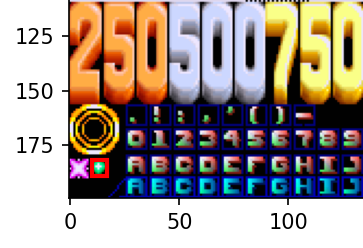
\includegraphics[width=12cm]{src/bullet/plot_detail.png}%
    \end{adjustbox}
\caption{The 'bullet' glyph located in the lower left in a red box.}
\end{figure}


The delightfully named routine '\icode{frab}' is responsible for \icode{f}i\icode{r}ing \icode{a b}ullet.
In here we can see the co-ordinates for plucking our bullet from the spritesheet being set. We define the
X and Y position within the sheet and the width and height too.

\begin{lstlisting}
frab:
    ; The bullet is taken from the sprite sheet in 'beasty3.cry'.
    ; This is an exception to the rule for nearly all other objects,
    ;  which are usually constructed polygons.
    ...
    move.l #$00b6000a,d0 ; Y (00b6) and X (000a) in sprite sheet 'pic'.
    move.l #$00070007,d1 ; Width (07) and height (07) for the bullet.
    ...
    move.l d0,36(a0)     ; Set the X/Y position in the sprite sheet.
    move.l d1,46(a0)     ; Set the width/height in the sprite sheet.
\end{lstlisting}

Notice how the Y and X values are encoded in a single 4-byte value:

\begin{lstlisting}
    move.l #$00b6000a,d0 ; Y (00b6) and X (000a) in sprite sheet 'pic'.
\end{lstlisting}
\begin{figure}[H]
  {
    \setlength{\tabcolsep}{3.0pt}
    \setlength\cmidrulewidth{\lightrulewidth} % Make cmidrule = 
    \begin{adjustbox}{width=3cm,center}
      \begin{tikzpicture}
      \def\BACKGROUNDONE{lightgreen}
      \def\BACKGROUNDTWO{lightblue}
      \fill[\BACKGROUNDONE] (0,0) rectangle ++ (1,1);
      \fill[\BACKGROUNDONE] (1,0) rectangle ++ (1,1);
      \fill[\BACKGROUNDTWO] (2,0) rectangle ++ (1,1);
      \fill[\BACKGROUNDTWO] (3,0) rectangle ++ (1,1);
        \draw[step=1.0,gray,thin] (0,0) grid (1,1);
        \node[matrix of math nodes,anchor=south west,inner sep=0pt,
        nodes={draw,minimum size=1cm,anchor=center},
        column sep=-\pgflinewidth,row sep=-\pgflinewidth,font=\huge\ttfamily]
        {
          00 & b6  & 00 & 0a \\
        };
      \end{tikzpicture}
    \end{adjustbox}
  \caption{Y of 182 (\icode{b6}) and X of 10 (\icode{0a}) encoded in a 4 byte long.}
  }
\end{figure}

Likewise the width and height:
\begin{lstlisting}
    move.l #$00070007,d1 ; Width (07) and height (07) for the bullet.
\end{lstlisting}
\begin{figure}[H]
  {
    \setlength{\tabcolsep}{3.0pt}
    \setlength\cmidrulewidth{\lightrulewidth} % Make cmidrule = 
    \begin{adjustbox}{width=3cm,center}
      \begin{tikzpicture}
      \def\BACKGROUNDONE{lightgreen}
      \def\BACKGROUNDTWO{lightblue}
      \fill[\BACKGROUNDONE] (0,0) rectangle ++ (1,1);
      \fill[\BACKGROUNDONE] (1,0) rectangle ++ (1,1);
      \fill[\BACKGROUNDTWO] (2,0) rectangle ++ (1,1);
      \fill[\BACKGROUNDTWO] (3,0) rectangle ++ (1,1);
        \draw[step=1.0,gray,thin] (0,0) grid (1,1);
        \node[matrix of math nodes,anchor=south west,inner sep=0pt,
        nodes={draw,minimum size=1cm,anchor=center},
        column sep=-\pgflinewidth,row sep=-\pgflinewidth,font=\huge\ttfamily]
        {
          00 & 07  & 00 & 07 \\
        };
      \end{tikzpicture}
    \end{adjustbox}
  \caption{Width of 7 (\icode{07}) and height of 07 (\icode{07}) encoded in a 4 byte long.}
  }
\end{figure}

With this setup complete, the routine \icode{draw\_pixex} on the opposite page will write these
values to the buffer used by the GPU routine 'rex'. With everything we have configured the result
will be to simply draw our selected segment from 'beasty3.cry' (i.e. our bullet) to the desired position on the screen.

I cheated earlier by shortening the \icode{frab} listing above. It actually contains an additional detail
where we can select a different type of bullet:
\begin{lstlisting}
frab:
    ; The bullet is taken from the sprite sheet in 'beasty3.cry'.
    ; This is an exception to the rule for nearly all other objects,
    ;  which are usually constructed polygons.
    ...
    move.l #$00b6000a,d0 ; Y (00b6) and X (000a) in sprite sheet 'pic'.
    move.l #$00070007,d1 ; Width (07) and height (07) for the bullet.
    tst 32(a0)           ; What type of bullet are we using?
    beq konk             ; If default, skip to konk.
    ; We're using the other bullet!
    move.l #$b60000,d0   ; Y (00b6) and X (0000) in sprite sheet 'pic'.
    move.l #$090009,d1   ; Width (09) and height (09) for the bullet.
konk:
    move.l d0,36(a0)     ; Set the X/Y position in the sprite sheet.
    move.l d1,46(a0)     ; Set the width/height in the sprite sheet.
\end{lstlisting}

For this alternate bullet, we select the sprite to the left of our previous bullet. Notice how the co-ordinates
and width/height are subtly altered for this version of the bullet.
\begin{lstlisting}
    move.l #$b60000,d0   ; Y (00b6) and X (0000) in sprite sheet 'pic'.
\end{lstlisting}
\begin{figure}[H]
  {
    \setlength{\tabcolsep}{3.0pt}
    \setlength\cmidrulewidth{\lightrulewidth} % Make cmidrule = 
    \begin{adjustbox}{width=3cm,center}
      \begin{tikzpicture}
      \def\BACKGROUNDONE{lightgreen}
      \def\BACKGROUNDTWO{lightblue}
      \fill[\BACKGROUNDONE] (0,0) rectangle ++ (1,1);
      \fill[\BACKGROUNDONE] (1,0) rectangle ++ (1,1);
      \fill[\BACKGROUNDTWO] (2,0) rectangle ++ (1,1);
      \fill[\BACKGROUNDTWO] (3,0) rectangle ++ (1,1);
        \draw[step=1.0,gray,thin] (0,0) grid (1,1);
        \node[matrix of math nodes,anchor=south west,inner sep=0pt,
        nodes={draw,minimum size=1cm,anchor=center},
        column sep=-\pgflinewidth,row sep=-\pgflinewidth,font=\huge\ttfamily]
        {
          00 & b6  & 00 & 00 \\
        };
      \end{tikzpicture}
    \end{adjustbox}
  \caption{Y of 182 (\icode{b6}) and X of 00 (\icode{00}) encoded in a 4 byte long.}
  }
\end{figure}

\begin{lstlisting}
    move.l #$090009,d1   ; Width (09) and height (09) for the bullet.
\end{lstlisting}
\begin{figure}[H]
  {
    \setlength{\tabcolsep}{3.0pt}
    \setlength\cmidrulewidth{\lightrulewidth} % Make cmidrule = 
    \begin{adjustbox}{width=3cm,center}
      \begin{tikzpicture}
      \def\BACKGROUNDONE{lightgreen}
      \def\BACKGROUNDTWO{lightblue}
      \fill[\BACKGROUNDONE] (0,0) rectangle ++ (1,1);
      \fill[\BACKGROUNDONE] (1,0) rectangle ++ (1,1);
      \fill[\BACKGROUNDTWO] (2,0) rectangle ++ (1,1);
      \fill[\BACKGROUNDTWO] (3,0) rectangle ++ (1,1);
        \draw[step=1.0,gray,thin] (0,0) grid (1,1);
        \node[matrix of math nodes,anchor=south west,inner sep=0pt,
        nodes={draw,minimum size=1cm,anchor=center},
        column sep=-\pgflinewidth,row sep=-\pgflinewidth,font=\huge\ttfamily]
        {
          00 & 09  & 00 & 09 \\
        };
      \end{tikzpicture}
    \end{adjustbox}
  \caption{Width of 9 (\icode{09}) and height of 09 (\icode{09}) encoded in a 4 byte long.}
  }
\end{figure}

The result is that we instead select the bullet sprite to the left of our original bullet:
\begin{figure}[H]
    \centering
    \begin{adjustbox}{width=9.5cm,center}
      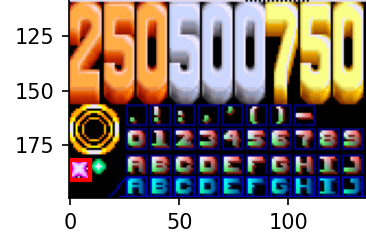
\includegraphics[width=12cm]{src/bullet/plot2_detail.png}%
    \end{adjustbox}
\caption{The alternate 'bullet' glyph located in the lower left in a red box.}
\end{figure}

